\documentclass[14pt,aspectratio=1610]{beamer}

\usepackage[brazil]{babel}
\usepackage[utf8]{inputenc}
%\UseRawInputEncoding
\usepackage[T1]{fontenc}
\usepackage{Sweave}
\usepackage{animate}
\usepackage{amsbsy}
\usepackage{amsfonts}
\usepackage{amsmath}
\usepackage{amssymb}
\usepackage{amsthm}
\usepackage[toc,page,title,titletoc]{appendix}
\usepackage[fixlanguage]{babelbib}
%\usepackage[pdftex]{color}
\usepackage{dsfont}
\usepackage{esvect}
\usepackage[labelfont=bf]{caption}
\usepackage{float}
\usepackage[Glenn]{fncychap}%Sonny %Conny %Lenny %Glenn %Renje %Bjarne %Bjornstrup
%\usepackage{geometry, calc, color, setspace}%
%\geometry{a4paper, headsep=1.0cm, footskip=1cm, lmargin=3cm, rmargin=2cm, tmargin=3cm, bmargin=2cm}
\usepackage{graphicx}
\usepackage{indentfirst}%Para indentar os parágrafos automáticamente
\usepackage{lipsum}
\usepackage{longtable}
\usepackage{mathtools}
\usepackage{listings}%Inserir codigo do R no latex
\usepackage{multirow}
\usepackage{multicol}
\usepackage{natbib}
\bibliographystyle{abbrvnat3}
\usepackage[figuresright]{rotating}
\usepackage{spalign}
%\usepackage{pgfpages}
\usepackage{pgfplots}
\usepackage{tikz}
\usepackage{color, colortbl}
\usepackage{ragged2e}%para justificar o texto dentro de algum ambiente
\definecolor{Gray}{gray}{0.9}
\definecolor{LightCyan}{rgb}{0.88,1,1}


\usepackage[all]{xy}
\usepackage{hyperref,bookmark}
\hypersetup{
  colorlinks=true,
  linkcolor=blue,
  citecolor=red,
  filecolor=blue,
  urlcolor=blue,
}

\usetheme{boxes}
%\usecolortheme[RGB={193,0,0}]{structure}

%\setbeamertemplate{footline}[frame number]
%\setbeamertemplate{footline}[text line]{%
%  \parbox{\linewidth}{\vspace*{-8pt}\hfill\date{}\hfill\insertshortauthor\hfill\insertpagenumber}}
\beamertemplatenavigationsymbolsempty
\renewcommand{\vec}[1]{\mbox{\boldmath$#1$}}
\newtheorem{Teorema}{Teorema}
\newtheorem{Proposicao}{Proposição}
\newtheorem{Definicao}{Definição}
\newtheorem{Corolario}{Corolário}
\newtheorem{Demonstracao}{Demonstração}
\newcommand{\bx}{\ensuremath{\bar{x}}}
\newcommand{\Ho}{\ensuremath{H_{0}}}
\newcommand{\Hi}{\ensuremath{H_{1}}}


\apptocmd{\frame}{}{\justifying}{} % Allow optional arguments after frame.

\title{MAF 261 - Estatística Experimental}
\author{Prof. Fernando de Souza Bastos}
\institute{Instituto de Ciências Exatas e Tecnológicas\texorpdfstring{\\ Universidade Federal de Viçosa}{}\texorpdfstring{\\ Campus UFV - Florestal}{}}
\date{2018}
\newcommand\mytext{Aula 9}
\newcommand\mytextt{Fernando de Souza Bastos}
\makeatletter
\setbeamertemplate{footline}
{
  \leavevmode%
  \hbox{%
  \begin{beamercolorbox}[wd=.333333\paperwidth,ht=2.25ex,dp=1ex,center]{author in head/foot}%
    \usebeamerfont{author in head/foot}\mytext
  \end{beamercolorbox}%
  \begin{beamercolorbox}[wd=.333333\paperwidth,ht=2.25ex,dp=1ex,center]{title in head/foot}%
    \usebeamerfont{title in head/foot}\mytextt
  \end{beamercolorbox}%
  \begin{beamercolorbox}[wd=.333333\paperwidth,ht=2.25ex,dp=1ex,right]{date in head/foot}%
    \usebeamerfont{date in head/foot}\insertshortdate{}\hspace*{2em}
    \insertframenumber{} / \inserttotalframenumber\hspace*{2ex} 
  \end{beamercolorbox}}%
  \vskip0pt%
}
\makeatother


\providecommand{\arcsin}{} \renewcommand{\arcsin}{\hspace{2pt}\textrm{arcsen}}
\providecommand{\sin}{} \renewcommand{\sin}{\hspace{2pt}\textrm{sen}}
%\newtheorem{Teorema}{Teorema}
%\newtheorem{Proposicao}{Proposição}
%\newtheorem{Definicao}{Definição}
%\newtheorem{Corolario}{Corolário}
%\newtheorem{Demonstracao}{Demonstração}

% Layout da pagina
\hypersetup{pdfpagelayout=SinglePage}
\begin{document}
\Sconcordance{concordance:Aula9.tex:Aula9.Rnw:%
1 129 1}


\frame{\titlepage}

\begin{frame}{}
\frametitle{\bf Sumário}
\tableofcontents
\end{frame}

\section{Introdução à Experimentação}
\begin{frame}{}
\frametitle{Introdução}
\begin{block}{}
\justifying
A experimentação tem por objetivo o estudo dos experimentos, isto é, seu planejamento, execução, análise dos dados obtidos e interpretação dos resultados.
\end{block}
\end{frame}

\begin{frame}{}
\frametitle{}
\begin{block}{}


\begin{columns}
        \column{7cm}
\justifying
{\bf Delineamento de Experimentos:} É o plano formal para conduzir o experimento. Inclui a escolha dos fatores, níveis, tratamentos e números de réplicas. Também pode ser entendido como a maneira como os tratamentos são designados às unidades experimentais.

        \column{6cm}
 \begin{block}{}

\pgfdeclareimage[height=5cm,width=6cm]{fig1}{Figuras/fig1}
\pgfuseimage{fig1}
\end{block}
\end{columns}
\end{block}
\end{frame}

\begin{frame}{}
\frametitle{}
\begin{block}{}
\justifying
Modelo geral de um processo para o delineamento de experimentos:
\begin{figure}[H]
    \centering
    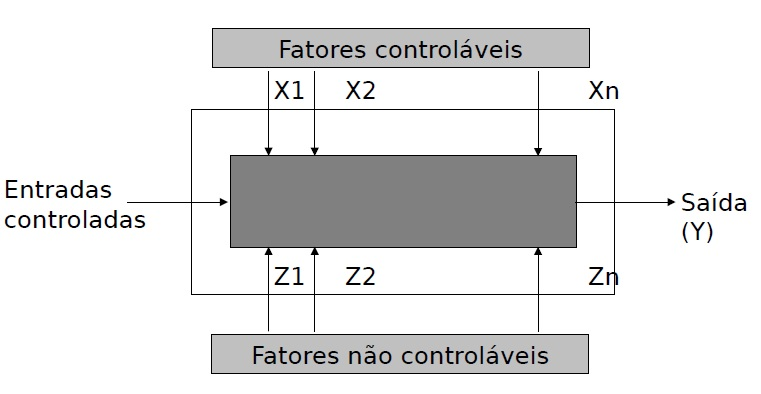
\includegraphics[scale=0.5]{Figuras/fig2}
    %\caption{}
    %\label{figRotulo}
  \end{figure}
\end{block}
\end{frame}

\begin{frame}{}
\frametitle{Exemplo 1}
\begin{block}{}
\justifying
Um banco está interessado em aumentar o lucro das suas agências e deseja saber qual é o tipo de propaganda mais eficiente. Seleciona, então, os veículos de propaganda a seguir: rádio, televisão, jornal e mala direta. Neste caso temos:

As {\bf entradas controladas} são os insumos do processo (todas as matérias-primas utilizadas)

Os {\bf fatores controláveis} são:
\begin{itemize}
\item Propaganda: tipos e valores a serem despendidos;\pause
\item Agências: Quantidade e localização;\pause
\item Funcionários: Quantidade em cada agência;\pause
\item Treinamento do pessoal: Assuntos, verbas, locais etc;\pause
\item Produtos oferecidos pelo banco e etc;
\end{itemize}
\end{block}
\end{frame}

\begin{frame}{}
\frametitle{Exemplo 1}
\begin{block}{}
\justifying
Os {\bf fatores não controláveis} são:
\begin{itemize}
\item Ações da concorrência;\pause
\item Ações governamentais;\pause
\item Crises ecônomicas mundiais;\pause
\item Crises ecônomicas nacionais;\pause
\item Greves e etc;
\end{itemize}

{\bf Saída} $(Y)$ é o lucro semestral do banco.

\end{block}
\end{frame}

\begin{frame}{}
\frametitle{}
\begin{block}{}
\justifying
Assim, o fator a ser testado é o veículo de propaganda, pois o banco está interessado em saber qual deles é mais eficiente (rádio, televisão, jornal ou mala direta) e qual a influência de cada um no seu lucro semestral, para poder depois investir adequadamente, proporcionando o maior retorno para os acionistas.
\end{block}
\end{frame}

\begin{frame}{}
\frametitle{}
\begin{block}{}
\justifying
Algumas questões podem ser levantadas:
\begin{itemize}
\item Os veículos de propaganda são os únicos a serem testados? Vamos ignorar outros, como a internet, outdoors, revistas e etc.?\pause
\item A influência dos fatores não controláveis pode ser grande? O que acontece se algum fator importante não puder ser controlado?\pause
\item A ordem de realização dos experimentos pode influenciar na conclusões?\pause
\end{itemize}
Essas questões precisam ser respondidas após a aplicação de uma série de experimentos!
\end{block}
\end{frame}

\begin{frame}{}
\frametitle{Exemplo 2}
\begin{block}{}
\justifying
Uma granja quer diminuir o tempo de engorda para abate dos seus frangos e dispõe de 4 tipos de ração para serem testados.
As {\bf entradas controladas} são os insumos do processo (Filhotes de frango, ração, água e medicamentos)

Os {\bf fatores controláveis} são:
\begin{itemize}
\item Tipo e quantidade diária de ração;\pause
\item Quantidade de aves por aviário;\pause
\item Raça dos animais;\pause
\item Bem-estar das aves.
\end{itemize}
\end{block}
\end{frame}

\begin{frame}{}
\frametitle{}
\begin{block}{}
\justifying
Os {\bf fatores não controláveis} são:
\begin{itemize}
\item Chuvas;\pause
\item Temperaturas;\pause
\item Ruídos;\pause
\item Características genéticas dos frangos.\pause
\end{itemize}

{\bf Saída} $(Y)$ peso das aves após certo número de dias.\pause

{\bf Obs:} Observe-se que todos os fatores poderiam ser controlados, mas isto não seria conveniente ou econômico, por isso a classificação dada, que levou em conta aspectos práticos!
\end{block}
\end{frame}

\begin{frame}{}
\frametitle{}
\begin{block}{}
\justifying
Deve-se variar o tipo de ração, mantendo-se fixos os outros fatores controláveis, para
verificar o efeito no tempo de engorda das aves, até que atinjam o peso de abate.
\end{block}
\end{frame}

\begin{frame}{}
\frametitle{}
{\bf Importante:} as aves que receberam a mesma ração terão uma certa variabilidade de peso, devido aos fatores não controláveis. Assim, algumas comerão mais do que outras ou terão maior aproveitamento do alimento, engordando mais do que as outras, devido a
fatores genéticos, por exemplo. \pause

\begin{block}{}
\justifying
{\bf A variabilidade é inerente aos processos em geral. Ela ocorrerá, inevitavelmente,
embora possa ser minimizada.}
\end{block}
\end{frame}

\begin{frame}{}
\frametitle{Conceitos Básicos}
\begin{block}{}
\justifying
\begin{itemize}
\item {\bf Fator:} É uma das causas (variáveis) que estão sendo estudados no experimento. Pode ser qualitativo ou quantitativo.\pause
\begin{itemize}
\item Quantitativo - Ex: Temperatura em $^{\circ}C,$ tempo em minutos etc.\pause
\item Qualitativo - Ex: diferentes operadores, diferentes máquinas, ligado ou desligado etc.
\end{itemize}
\end{itemize}
\end{block}
\end{frame}

\begin{frame}{}
\frametitle{}
\begin{block}{}
\justifying
\begin{itemize}
\item {\bf Níveis do fator:} São os diferentes valores do fator que são escolhidos para o experimento. \pause
\item {\bf Tratamento:} É um nível único assinalado para um fator durante um experimento. Exemplo: Temperatura de $50^{\circ}C$. Uma combinação de tratamentos é o conjunto de todos os fatores utilizados num determinado ensaio. Exemplo: ensaio usando o operador João, máquina A e temperatura de $50^{\circ}C$.
\end{itemize}
\end{block}
\end{frame}

\begin{frame}{}
\frametitle{}
\begin{block}{}
\justifying
\begin{itemize}
\item {\bf Ensaio:} É cada realização do experimento em uma determinada combinação de tratamentos. O experimento é constituído pelo conjunto de todos os ensaios realizados nas diversas combinações de tratamentos, com as várias réplicas.\pause
\item {\bf Réplicas:} São as repetições de um experimento executadas nas mesmas condições experimentais.\pause
\item {\bf Unidade experimental:} é a unidade que vai receber o tratamento e fornecer os dados que deverão refletir o seu efeito. Exemplos: a) uma fileira de plantas com 3
metros de comprimento no campo; b) um leitão e c) um litro de leite.
\end{itemize}
\end{block}
\end{frame}

\begin{frame}{}
\frametitle{}
\begin{block}{}
\begin{itemize}
\item {\bf Esquema:} quando em um mesmo experimento são avaliados dois ou mais fatores
os níveis dos fatores podem ser combinados de maneiras diferentes. O esquema é
justamente a maneira utilizada pelo pesquisador ao combinar os níveis dos fatores
para se obter os tratamentos.\pause
\item {\bf Variável resposta:} é a variável mensurada usada para avaliar o efeito de
tratamentos.\pause
\item {\bf Erro experimental:} é o efeito de fatores que atuam de forma aleatória e 
que não são passíveis de controle pelo experimentador.
\end{itemize}
\end{block}
\end{frame}

\section{Princípios Básicos da Experimentação}
\subsection{Princípio da Repetição}
\begin{frame}{}
\frametitle{Princípio da Repetição}
\begin{block}{}
\justifying
A repetição consiste em aplicar o mesmo tratamento a várias unidades
experimentais, ou seja, consiste na reprodução do experimento básico.\pause
\begin{itemize}
\item Não existe regra para limitar o número mínimo de repetições.\pause
\item Sugere-se que os experimentos tenham pelo menos 20 unidades experimentais e 10 graus de liberdade para o resíduo.\pause
\item Quanto maior o número de repetições, maior a precisão do experimento.\pause
\item {\bf O uso do princípio da repetição tem por finalidade obter uma estimativa do erro experimental.}
\end{itemize}
\end{block}
\end{frame}

\subsection{Princípio da Casualização}
\begin{frame}{}
\frametitle{Princípio da Casualização}
\begin{block}{}
\justifying
O princípio da casualização consiste em distribuir ao acaso os tratamentos às
unidades experimentais. Com o uso do princípio da casualização, as variações que contribuem para o erro experimental são convertidas em variáveis aleatórias.
\end{block}
\end{frame}

\begin{frame}{}
\frametitle{}
\begin{block}{}
\justifying
Do ponto de vista estatístico, com o uso do princípio da casualização em um
experimento:
\begin{enumerate}
\item Obtém-se uma estimativa válida do erro experimental;\pause
\item Fica garantido o uso de testes de significância, pois os erros experimentais
atuam de forma independente nas diversas unidades experimentais.\pause
\end{enumerate}
{\bf Todo experimento deve conter no mínimo os princípios básicos da repetição e da
casualização.}
\end{block}
\end{frame}

\subsection{Princípio do Controle na Casualização}
\begin{frame}{}
\frametitle{Princípio do Controle na Casualização}
\begin{block}{}
\justifying
O uso do princípio do controle na casualização só é recomendado quando as unidades experimentais não são ou não estão sob condições homogêneas devido a influência de um ou mais fatores. Para utilizar este princípio, é necessário inicialmente dividir as unidades experimentais em blocos de unidades de tal forma que dentro de cada bloco haja homogeneidade e um número de unidades igual ao número de tratamentos do experimento. A distribuição dos tratamentos as unidades é feita então dentro de cada bloco. Daí o nome do princípio {\it controle} na casualização.
\end{block}
\end{frame}

\begin{frame}{}
\frametitle{}
\begin{block}{}
\justifying
A finalidade, do uso do princípio do controle na casualização, é reduzir o efeito do
erro experimental através do controle da variação existente entre as unidades experimentais. Espera-se que com o controle na casualização a estimativa obtida para o erro experimental seja menor.
\end{block}
\end{frame}

\section{Fontes de variação de um experimento}
\begin{frame}{}
\frametitle{}
\begin{block}{Em um experimento podem ocorrer as seguintes fontes de variação:}
\begin{itemize}
\item {\bf Premeditada}
\end{itemize}
É aquela introduzida pelo pesquisador com a finalidade de fazer comparações. Por
exemplo: tratamentos.\pause
\begin{itemize}
\item {\bf Sistemática}
\end{itemize}
Variações não intencionais, mas de natureza conhecida. Podem ser controladas pelo pesquisador. Por exemplo: heterogeneidade do solo, tamanho de semente, etc.\pause
\begin{itemize}
\item {\bf Aleatória}
\end{itemize}
São variações de origem desconhecida, não podendo ser controladas. Constituem
o erro experimental. São devidas a: variações no material experimental e falta de uniformidade nas condições experimentais.
\nocite{calegare}
\nocite{ivo}
\end{block}
\end{frame}

\begin{frame}[allowframebreaks]
\frametitle{Referências Bibliográficas}
\bibliography{bibliografia}
\end{frame}

\end{document}
